%Wir verwenden eine DIN-A4-Seite und die Schriftgröße 12.
\documentclass[a4paper,12pt]{scrartcl} 


%Diese drei Pakete benötigen wir für die Umlaute, Deutsche Silbentrennung etc.
%Apple-Nutzer sollten anstelle von \usepackage[latin1]{inputenc} das Paket \usepackage[applemac]{inputenc} verwenden
%% \usepackage[latin1]{inputenc}
%%apt-get install texlive-lang-german damit ngerman keine Probleme mehr macht !!
%\usepackage[utf8]{inputenc} 
%\usepackage[T1]{fontenc}
%\usepackage[ngerman]{babel}

%Das Paket erzeugt ein anklickbares Verzeichnis in der PDF-Datei.
%\usepackage{hyperref}

%Das Paket wird für die anderthalb-zeiligen Zeilenabstand benötigt
\usepackage{setspace}

%%HTWM-Vorlage - benoetigt apt-get install texlive-fonts-extra
\setcounter{tocdepth}{3}				%Schatelungstiefe Inhaltsverz.
\usepackage[utf8]{inputenc}			%deutsche Umlaute
\usepackage[ngerman]{babel}			%Rechtschreibprüfung
\usepackage{color,listings} 			%Quellcode Highlighting, bindet das
%Paket Listings ein
\usepackage{listings}
\usepackage{color}
\usepackage{textcomp}
\usepackage[T1]{fontenc}				%srccode
\usepackage[scaled]{beramono}		%srccode
\usepackage{longtable}				%mehrseitige tabellen
\usepackage[tableposition=b]{caption}
\usepackage[pdftex, pdftoolbar=false, hyperfootnotes=false, bookmarks,
bookmarksopen, bookmarksnumbered, bookmarksopenlevel=2, pdfpagelabels=true,
pdfstartpage=3, pdfstartview=FitH,]{hyperref} %Verlinkungen
\usepackage{array}					%farbige Tabellen
\usepackage[table]{xcolor} 			%farbige Tabellen
\usepackage{graphicx}				% \includegraphics bnoetigt dies
\usepackage{draftwatermark}			% wasserzeichen
	%Quelle: http://choorucode.com/2010/05/05/latex-adding-draft-watermark/?like=1&source=post_flair&_wpnonce=1c9f85538d
\SetWatermarkText{VORABVERSION}		% wasserzeichen-text
\SetWatermarkLightness{0.9}			% wasserzeichen-kontrast
\SetWatermarkScale{2.5}				% wasserzeichen-zeichengroe\ss{}e

\definecolor{Navy}{rgb}{0,0,0.5}
\definecolor{Gray}{gray}{0.5}
\definecolor{dunkelgrau}{rgb}{0.8,0.8,0.8}
\definecolor{hellgrau}{rgb}{0.95,0.95,0.95}
\definecolor{hellgrau2}{rgb}{0.93,0.93,0.93}

\hypersetup{
	colorlinks=true, 			% false: boxed links; true: colored links
	linkcolor=Navy,          		% color of internal links
	citecolor=Gray,        			% color of links to bibliography
	filecolor=magenta,      		% color of file links
	urlcolor=blue,           			% color of external links
	linkbordercolor={1 1 1}, 		% set to white
	citebordercolor={1 1 1} 		% set to white
}


%Einrückung eines neuen Absatzes
\setlength{\parindent}{0em}

%Definition der Ränder
\usepackage[paper=a4paper,left=30mm,right=30mm,top=30mm,bottom=30mm]{geometry} 

%Abstand der Fussnoten
\deffootnote{1em}{1em}{\textsuperscript{\thefootnotemark\ }}

%Regeln, bis zu welcher Tiefe (section,subsection,subsubsection) Überschriften angezeigt werden sollen (Anzeige der Überschriften im Verzeichnis / Anzeige der Nummerierung)
%\setcounter{tocdepth}{3}
%\setcounter{secnumdepth}{3}



\begin{document}

%Beginn der Titelseite
\begin{titlepage}
\begin{small}
\vfill {HTWK Leipzig\\ 
Fachbereich IMN \\ 
Wintersemester 2012/2013}
\end{small}


\begin{center}
\begin{Large}
\vfill {\textsf{\textbf{
Ausarbeitung zum Fach Message-Passing-Programmierung\\--VORABVERSION--\\
}}}
\end{Large}
Beleg im Fach Message-Passing-Programmierung
\end{center}

\begin{small}
\vfill
Kurt Junghanns\\Philipp-Rosenthal-Stra\ss{}e 32\\04103 Leipzig\\kurt.junghanns@stud.htwk-leipzig.de\\
\\Marcel Kirbst\\Sieglitz 39\\06618 Molau\\marcel.kirbst@stud.htwk-leipzig.de\\ \\
\today
\end{small}

\end{titlepage}
%Ende der Titelseite


%Inhaltsverzeichnis (aktualisiert sich erst nach dem zweiten Setzen)
\tableofcontents
\thispagestyle{empty}

%Beginn einer neuen Seite
\clearpage

%Anderthalbzeiliger Zeilenabstand ab hier
\onehalfspacing

\pagestyle{plain}


\section{Einleitung}
Diese Ausarbeitung ist das Resultat der Veranstaltung Message-Passing-Programmierung im Wintersemester 2012/2013 und pr\"asentiert die eingereichten Programme
als Grundlage der m\"undlichen Pr\"ufung der Pr\"uflinge Kurt Junghanns und Marcel Kirbst.

Die Aufgabenstellung erfordert die Bearbeitung von zwei Aufgaben, die auf unterschiedlichen Hardware-Plattformen zu implementieren waren.

%% IMPORT PDF GRAPHIC AS VECTOR GRAPHIC
%\begin{figure}[htb]
%\begin{center}
% \includegraphics[width=1\hsize]{./images/default.pdf}
% % test.pdf: 595x842 pixel, 72dpi, 20.99x29.70 cm, bb=0 0 595 842
%\end{center}
%\caption[Beispielhafte Standardkonfiguration eines Internetanschlu\ss{}, Quelle: Autor, verwendete Symbole unterliegen der
%GPL]{\label{stdinet}Beispielhafte Standardkonfiguration eines Internetanschlu\ss{}.}
%\end{figure}


%% EXAMPLE TABLE: longtable, colored columns and rows and description under table
%\begin{longtable}{p{34mm}>{\columncolor[gray]{0.97}}p{33mm}p{33mm}>{\columncolor
%[gray]{0.97}}p{33mm}}
%\rowcolor[gray]{.9}Funktion & \textbf{IPCop} & \textbf{IPFire} &
%\textbf{pfSense}\\
%Lizenz & GPL & GPL & BSD\\
%\rowcolor[gray]{.95}Betriebssystem & Linux & Linux & FreeBSD   \\
%Hardware"-architektur & i386, Cobald, Sparc, PowerPC & i386,
%AMD64 & i386, AMD64\\
%\rowcolor[gray]{.95}vorkonfigurierte Pakete & nein & ja & ja \\
%eigene Paketverwaltung & nein & nein & ja \\
%\rowcolor[gray]{.95}Automatisches Update & nein & nein & ja \\
%VLAN-Unterst\"utzung & nein & nein & ja mit entsprechenden
%Netzwerkkarten\\
%\rowcolor[gray]{.95}Netzwerkschnittstellen & max. 4 & max. 4 & nur durch
%Hardware begrenzt \\
%\caption{Merkmale der Routerdistributionen im Vergleich}
%\label{Merkmale der Routerdistributionen im Vergleich}
%\end{longtable}

\section{Message-Passing-Interface (MPI)}

\subsection{Aufgabenstellung / Problembeschreibung}
Die empfohlene Aufgabenstellung f\"ur die MPI-Teilaufgabe ist die Implementierung eines so genannten Merge-Splitting-Sort-Algorithmus, der eine vorzugebende
Anzahl nat\"urlicher Zahlen in zuf\"alliger Reihenfolge auf einer vorzugebenden Anzahl an Prozessoren sortiert. Dabei soll die ben\"otigte Laufzeit ermittelt
werden um im Anschlu\ss{} Aussagen \"uber das Laufzeitverhalten der Implementierung in Abh\"angigkeit zur verwendeten Element- und Prozessorzahl treffen zu
k\"onnen.

Dieser Algorithmus wurde in einem C-Programm unter Zuhilfenahme der MPI Bibliothek umgesetzt.
Nachfolgend werden Aussagen zum Laufzeitverhalten getroffen. Dabei wurden den Laufzeitmessungen die Anzahl zu sortierender Elemente wie in der Aufgabenstellung
empfohlen mit 20.000, 40.000 sowie 80.000 Elementen zu Grunde gelegt.

\subsection{Programmbeschreibung}
Zun\"achst wird ein Array mit n Zufallszahlen von jedem Prozess erzeugt. Dieses wird sortiert, wobei die lokale Prozessorlaufzeit T(1) ermittelt wird. Jeder
Prozessor erzeugt n/p Zufallszahlen und speichert sie in einem Array ab, wobei p die Anzahl der verwendet Prozessoren angibt. Die Kommunikation zwischen den
Prozessoren wird durch die Funktionen \texttt{MPI\_Send()} und \texttt{MPI\_Recv()} realisiert. Die Zeiterfassung erfolgt dabei mit der
Funktion \texttt{MPI\_Wtime()}. Anschlie\ss{}end wird der Merge-Splitting-Sort-Algorithmus ausgef\"uhrt. Nach diesem verteilten Sortiervorgang ermittelt jeder
Prozessor die ben\"otigten Messwerte:
\begin{itemize}
 \item Gesamtlaufzeit
 \item Speedup
 \item Anteil der initialen Phase
 \item Kommunikationsanteil
\end{itemize}
Ein ausgezeichneter Prozessor sammelt die erfassten Werte und die sortierten Arrays ein und ermittelt die Durchschnittswerte. Dies erfolgt mit Hilfe der
Funktionen \texttt{MPI\_Reduce()} und \texttt{MPI\_Gather()}. Dieser Prozessor ist au\ss{}erdem f\"ur die Ausgabe der Resultate auf der Konsole zust\"andig.

Bei Aufruf erwartet das Programm folgendene Startparameter:
\begin{description}
 \item [n:]  Gr\"o\ss{}e des Gesamtarray an zu sortierenden Elementen, wobei der Wert n ein ganzzahliges Vielfaches der verwendeten
Prozessoranzahl sein muss
 \item [k:]  (optional) Die \"Ubergabe dieses Parameters bewirkt zus\"atzliche Ausgabe des sortierten Arrays
\end{description}

Der vollst\"andige Quellcode des Programms sowie aller Skripte liegt dem Projektordner und ist au\ss{}erdem aus dem \"offentlichen Repository unter
\footnote{\url{https://github.com/mkirbst/mpp_mpi}} abrufbar.

\subsection{Laufzeitumgebung}
Um die Entwicklung und die Tests der Implementierung so effektiv wie m\"oglich zu gestalten, wurden mehrere BASH-Skripte erstellt.
Das BASH-Skript \texttt{run.sh}, dass im Anhang vollst\"andig aufgef\"uhrt ist,  erf\"ullt dabei die folgenden Funktionen:
\begin{itemize}
 \item Ermitteln der Prozessoranzahl \textbf{p}, Anzahl der zu sortierenden Elemente \textbf{n}, Name der zu kompilierenden C-Datei, Name der kompilierten
Bin\"ardatei als Startparameter
 \item pr\"ufen, welcher der Rechner im Pool per SSH erreichbar sind
 \item ermitteln der durchschnittlichen Auslastung aller errichbaren Rechner im Pool
 \item sortieren der erreichbaren Poolrechner aufsteigend nach der durchschnittlichen Auslastung der letzten Minute, der letzten 5 Minuten, der letzten 15
Minuten
 \item Kompilieren der angegebenen C-Datei
 \item Ausf\"uhrung der resultierenden Bin\"ardatei auf den \textbf{p} Rechnern mit der geringsten durchschnittlichen Auslastung um das Risiko einer
Verf\"alschung der Messergebnisse durch Fremdeinwirkung zu minimieren
\end{itemize}

Ein weiteres weiteres BASH-Skript \texttt{bench.sh} ruft die Bin\"ardatei mit den empfohlenen Elementanzahlen 20.000, 40.000 und 80.000 sequentiell f\"ur 2, 4,
8, 10, 16 und 20 Prozessoren auf und gibt die jeweils gemessenen Zeitintervalle \"ubersichtlich aus um eine grafische Auswertung mit g\"angigen
Tabellenkalkulationsprogrammen zu gestatten. 

\subsection{Ergebnisse und Auswertung}

\subsubsection{Initiale Phase}
\begin{figure}[htb]
  \begin{center}
    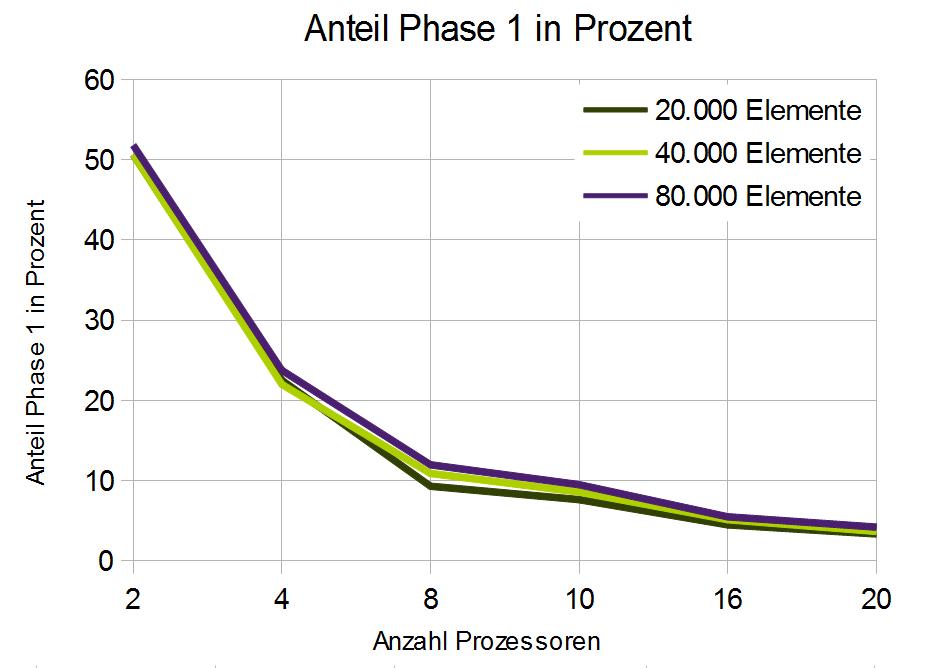
\includegraphics[width=1\hsize]{../Anteil_Phase_1.PNG}
  \end{center}
  \caption{\label{mpiphaseeins}
    Phase-1-Diagramm f\"ur die MPI-Implementierung}
\end{figure}
In der Initialphase des Merge-Splitting-Sort-Algorithmus wird das lokale Array eines jeden Prozessors initial sortiert. Da die Initialphase im Gegensatz zu den
nachfolgenden Phasen unabh\"angig von der Anzahl der genutzen Prozessoren immer nur einmalig durchlaufen wird, sinkt der Anteil der Initialphase an der
Gesamtlaufzeit des Algorithmus mit steigender Prozessoranzahl. W\"ahrend sich bei der Nutzung von nur zwei Prozessoren noch ein Laufzeitanteil der Phase 1 von
50 Prozent ergibt, sinkt dieser Wert bei Nutzung von 10 Prozessoren schon auf unter 10 Prozent, Tendenz weiter fallend.

\subsubsection{Speedup}
\begin{figure}[htb]
  \begin{center}
    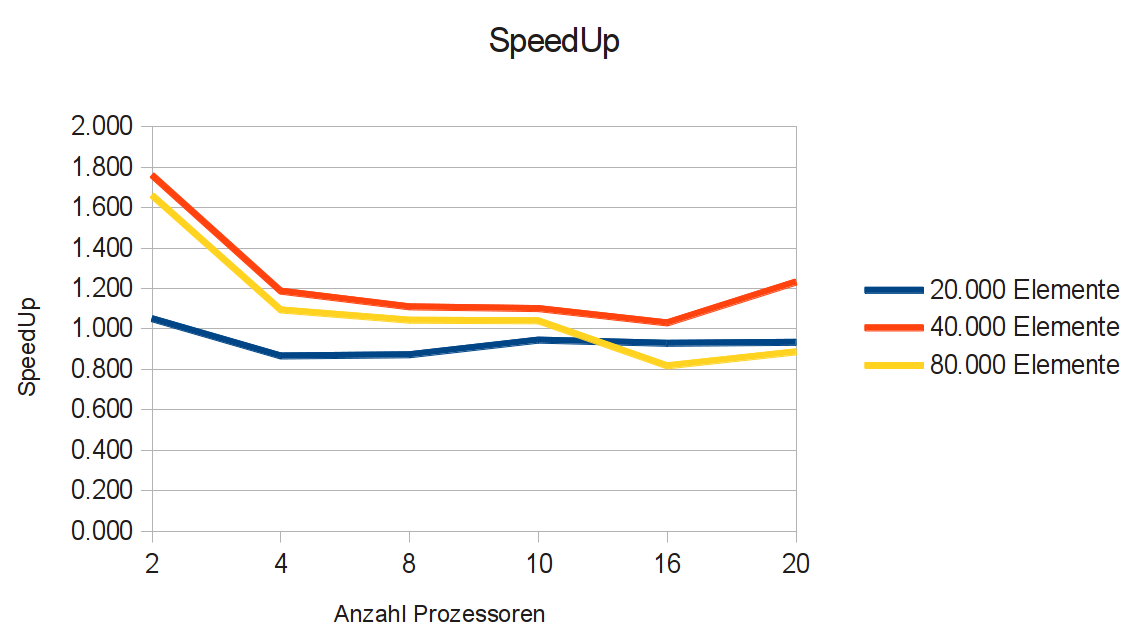
\includegraphics[width=1\hsize]{../speedup.png}
  \end{center}
  \caption{\label{mpispeedup}
    Speedup-Diagramm f\"ur die MPI-Implementierung}
\end{figure}
Der Speedup ist der Quotient aus der Laufzeit des Algorithmus bei der Nutzung eines Prozessors und der Laufzeit bei Nutzung mehrerer Prozessoren.
Ein Speedup-Wert von 1 sagt aus, dass der Algorithmus auf einem Prozessor der Laufzeit des Algorithmus auf mehreren Prozessoren entspricht.
Im Idealfall steigt der Speedup proportional mit der Anzahl der Prozessoren. \\\\

Nach Ahmdal setzt sich die Gesamtlaufzeit des parallelisierten Algorithmus zusammen aus einem Anteil mit nichtparallelisierbaren Code (sog.: sequenzieller
Anteil) und einem Anteil an parallelisierbaren Code, dessen Laufzeit sich umgekehrt proportional zur Anzahl der benutzten Prozessoren verhält.
Ahmdals Gesetz berücksichtigt hierbei jedoch nicht den mit steigender Prozessoranzahl ebenfalls wachsenden Kommunikationsaufwand. \\\\

Das zu erwartende Laufzeitverhalten für reale Implementierungen legt daher nahe, das der Speedup nicht linear mit der Anzahl der eingesetzten Prozessoren
ansteigt, sondern auf Grund des ebenfalls ansteigenden Kommunikationsaufwandes ab einer bestimmten Prozessoranzahl wieder abnimmt. \\ \\

Die durchgeführten Laufzeitmessungen mit der Implementierung des Algorithmus zeigen jedoch, dass bereits bei Nutzung von mehr als 10 Prozessoren der Speedup mit
steigender
Prozessoranzahl abnimmt. Der im Test beste erreichte Speedup stellte sich bei Nutzung von 10 Prozessoren und hinreichend vieler Elemente ein (>= 80.000).
Bereits beim Einsatz von von 16 Prozessoren war die Laufzeitverringerung gegenüber der vollständig sequenziellen Implementierung nur noch marginal, Tendenz
abnehmend. Dieses von den theoretisch erwarteten Messwerten abweichende Laufzeitverhalten ist das Ergebnis weiterer Einflussfaktoren wie beispielsweise:
\begin{itemize}
  \item Eingesetzte Hardware (Netzwerkstruktur, nicht exklusiv genutzte Hardware )
  \item Eingesetzte Software (Betriebssystem, genutze Implementierung des Message-Passing-Interface)
  \item Implementierung des Algorithmus (eingesetzter Sortieralgorithmus, Kommunikationsablauf)
\end{itemize}
Im Laufe der Implementation wurde ein direkter Einfluss des verwendeten Sortieralgorithmus auf die Gesamtlaufzeit deutlich. Es wurden  verschiedene
Quicksort-Implementationen getestet, wobei durch die in der Standardbibliothek von C enthaltene Funktion \texttt{qsort()} die besten Ergebnisse liefert.

\subsubsection{Effizienz}
\begin{figure}[htb]
  \begin{center}
    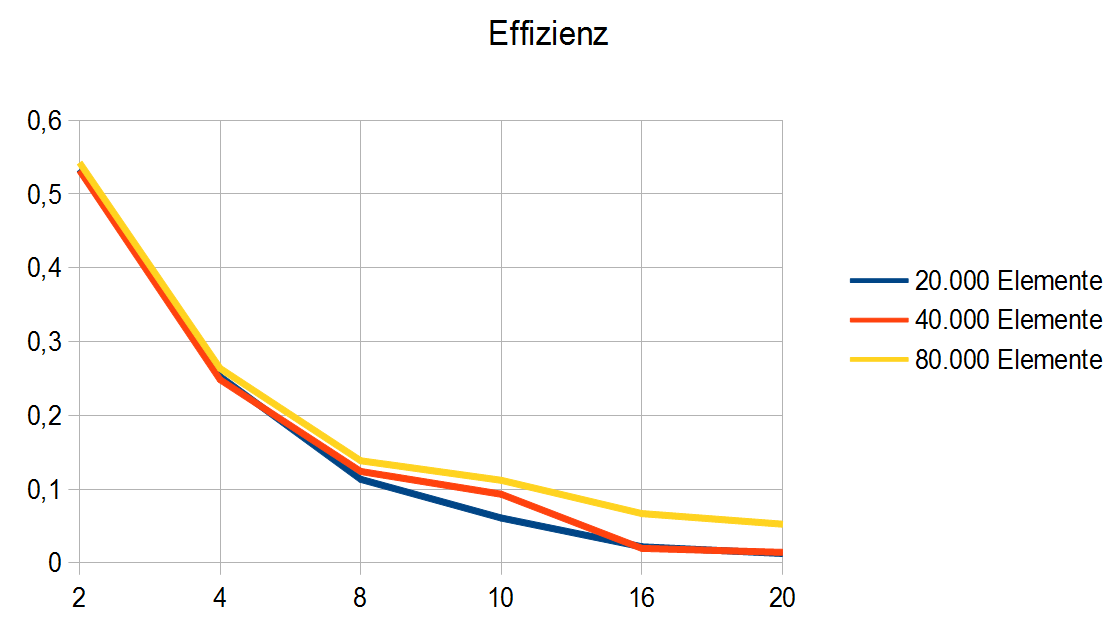
\includegraphics[width=1\hsize]{../effizienz.png}
  \end{center}
  \caption{\label{mpieffizienz}
    Effizienz-Diagramm f\"ur die MPI-Implementierung}
\end{figure}
Eine weiterer aussagekräftiger Wert ist die Effizienz.
Die Effizienz gibt die relative Verbesserung in der Verarbeitungsleistung an und ergibt sich aus dem Quotient von Speedup und Prozessoranzahl.
Wie aus dem betreffenden Diagramm ersichtlich wird, nimmt die Effizienz umgekehrt proportional zur Anzahl der eingesetzten
Prozessoren ab. Dabei hat die Anzahl der zu sortierenden Elemente nur marginalen Einfluss auf die jeweiligen Effizienzwerte. 

\subsubsection{Kommunikationsanteil}
\begin{figure}[htb]
  \begin{center}
    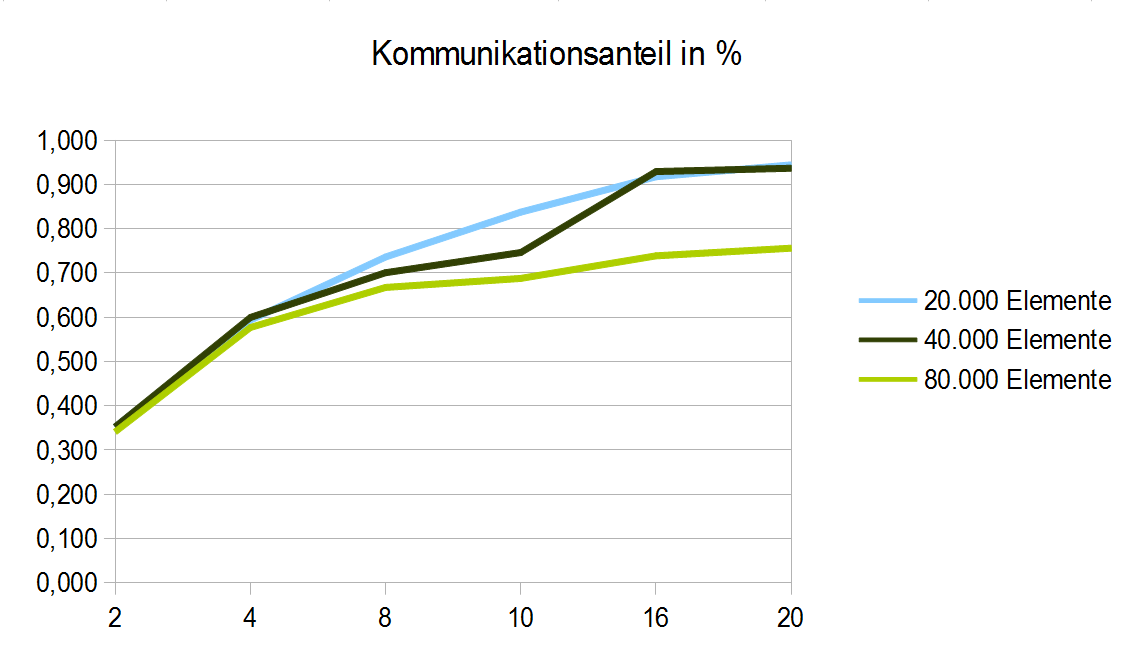
\includegraphics[width=1\hsize]{../Kommunikationsanteil.PNG}
  \end{center}
  \caption{\label{mpikommoverhead}
    Diagramm des Kommunikationsanteils f\"ur die MPI-Implementierung}
\end{figure}
Die Auswertung der Messwerte zeigt, dass mit steigender Anzahl zu sortierender Elemente der Kommunikationsanteil an der Gesamtlaufzeit exponentiell ansteigt.
Bereits bei Verwendung von 8 Prozessoren betr\"agt der Kommunikationsanteil an der Gesamtlaufzeit etwa 70 Prozent und steigt weiter an, sodass schon
f\"ur 20 Prozessoren der Kommunikationsanteil \"uber 80 Prozent mit weiterhin steigender Tendenz betr\"agt.
Dieser hohe Anteil der Kommunikation an der Gesamtlaufzeit ist durch die in 2.4.2 aufgez\"ahlten Einflussfaktoren, besonders aber auf die Netzwerkstruktur und
und MPI Implementierung, zur\"uckzuf\"uhren.\\\\

Zusammenfassend kann die Aussage getroffen werden, dass die Implementierung des Merge-Splittung-Sort Algorithmus unter der MPI-Umgebung nicht geeignet ist.\\
Die unter bestimmten Voraussetzungen zu erreichende maginale Verk\"urzung der Gesamtlaufzeit ist gering, sodass vor der konkreten Nutzung dieser
Implementierung im vornherein betrachtet werden muss, ob die Anzahl der Prozessoren und zu sortierenden Elemente zu einer Verbesserung der Gesamtlaufzeit
f\"uhrt.


\section{Parallelrechnersystem MC-3}
\subsection{Aufgabenstellung / Problembeschreibung}
F\"ur das Parallelrechnersystem MC-3 wurde die Aufgabe der nummerischen Integration mittels Parabelformel gew\"ahlt. Hierbei sollen Funktionen mit Hilfe der
Parabelformel \"uber einem gegebenen Intervall parallel von mehreren Rechenkernen nummerisch integriert werden.\\
Vorgegeben waren zu diesem Zweck folgende Funktionen:
\begin{itemize}
 \item $f(x) = x*sin(x)$ in dem Intervall von 0 bis $\pi$
 \item $f(x) = \frac{4}{x^2+1}$ in dem Intervall von 0 bis 1
\end{itemize}
Das Ergebnis der Integration soll $\pi$ sein. Dabei soll das Maschinen-$\pi$ mit doppelter Genauigkeit als Referenz f\"ur die Pr\"azision der Berechnung
dienen. Dies wurde in einem C-Programm umgesetzt. Die Anzahl der Prozessoren, die zu integrierende Funktion und die Anzahl der Zerlegungen des Intervalls sollen
dabei Eingabewerte sein. Als Resultat soll das Programm das Laufzeitverhalten und die Genauigkeit der Funktionen messen.

\subsection{Programmbeschreibung}
Das Programm wird auf dem Rechner Abel im Rechnerpool gestartet, der mit dem Multiprozessorsystem MC-3 verbunden ist. Als Startparameter muss \texttt{n} und
die Nummer der zu nutzenden Funktion \"ubergeben werden. \texttt{n} wird intern mit 8 multipliziert, um die Teilbarkeit mit der Prozessoranzahl zu
gew\"ahrleisten. Der Funktionsnummer 1 ist $f(x) = \frac{4}{x^2+1}$ zugeordnet und 2 der Funktion $f(x) = x*sin(x)$.\\

Die Zeiterfassung findet mit der Funktion \texttt{TimeNowHigh()} statt. Die Kommunikation hingegen mit \texttt{Send()} und \texttt{Recv()}.\\
F\"ur die Anordnung der Prozessoren wurde ein Stern gew\"ahlt. Dabei werden Links von allen Prozessoren mit der ID ungleich 0 zum Prozessor mit der ID 0
angelegt und verwendet.\\

Nach Auswertung der Argumente, ermittelt jeder Prozessor die Laufzeit f\"ur die sequentielle Berechnung des Integrals T(1).\\
Anschlie\ss{}end ermittelt jeder Prozessor das Integral seines Teilintervalls.
Schlussendlich empf\"angt der Prozessor mit der ID 0 alle ermittelten Teilintegrale sowie die Gesamtlaufzeit, T(1) und die zur
Kommunikation ben\"otigte Zeit.
Der Prozessor mit der ID bildet aus den Zeitwerten Durchschnitte und gibt sie in der Konsole aus.


\subsection{Laufzeitumgebung}
Hier ist nur ein Skript zur Erfassung der Messwerte f\"ur verschiedene Prozessoranzahlen, Intervallteilungen pro Prozessor und Funktionen zu nennen.\\
Dieses Skript ist im Anhang \nameref{mc3:erfassungsh} zu finden.\\\\


\subsection{Ergebnisse}
\subsubsection{Speedup}
\begin{figure}[htb]
  \begin{center}
    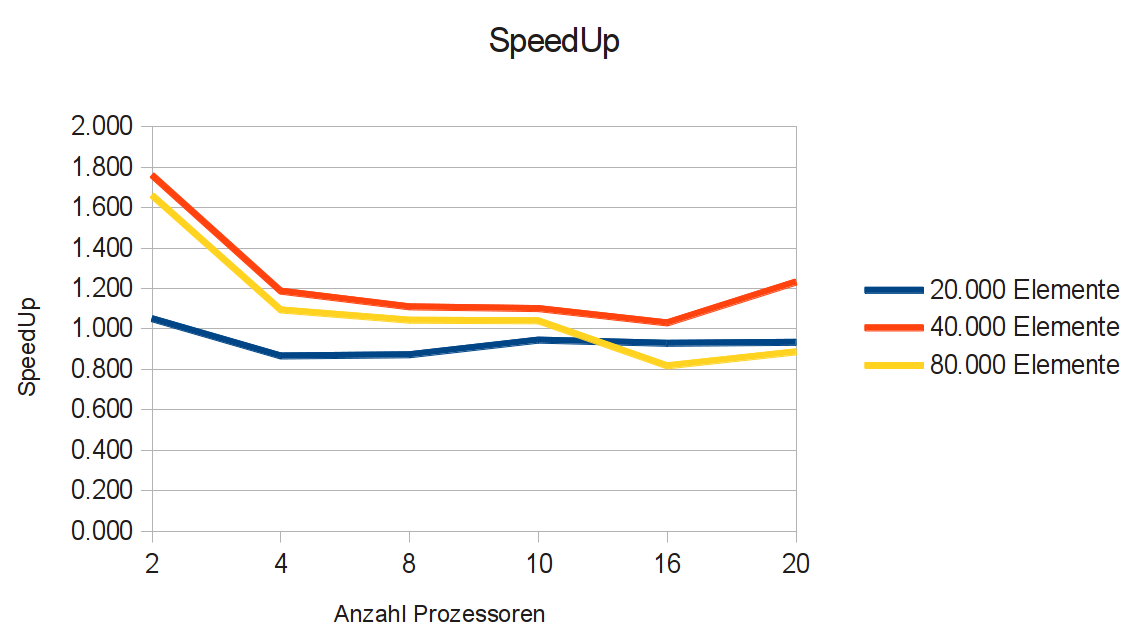
\includegraphics[width=1\hsize]{../speedup.png}
  \end{center}
  \caption{\label{mpispeedup}
    Speedup-Diagramm f\"ur die MC-3-Implementierung mit der Funktion 1}
\end{figure}
\begin{figure}[htb]
  \begin{center}
    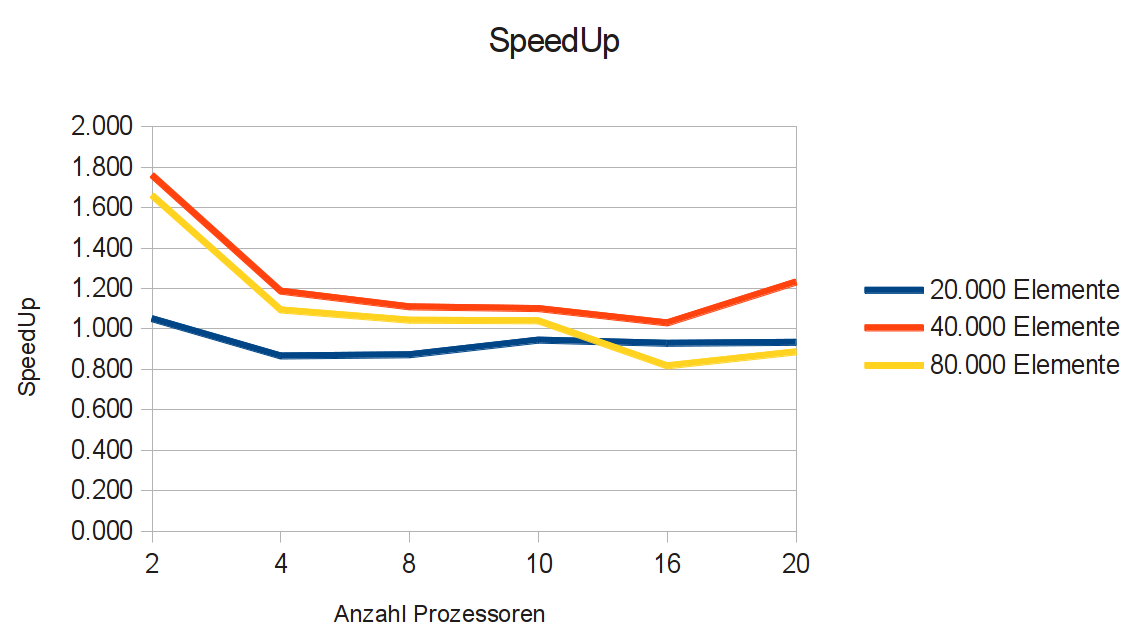
\includegraphics[width=1\hsize]{../speedup.png}
  \end{center}
  \caption{\label{mpispeedup}
    Speedup-Diagramm f\"ur die MC-3-Implementierung mit der Funktion 2}
\end{figure}
Die durchgeführten Laufzeitmessungen mit der Implementierung des Algorithmus zeigen jedoch, dass bereits bei Nutzung von mehr als 10 Prozessoren der Speedup mit
steigender
Prozessoranzahl abnimmt. Der im Test beste erreichte Speedup stellte sich bei Nutzung von 10 Prozessoren und hinreichend vieler Elemente ein (>= 80.000).
Bereits beim Einsatz von von 16 Prozessoren war die Laufzeitverringerung gegenüber der vollständig sequenziellen Implementierung nur noch marginal, Tendenz
abnehmend. Dieses von den theoretisch erwarteten Messwerten abweichende Laufzeitverhalten ist das Ergebnis weiterer Einflussfaktoren wie beispielsweise:
\begin{itemize}
  \item Eingesetzte Hardware (Netzwerkstruktur, nicht exklusiv genutzte Hardware )
  \item Eingesetzte Software (Betriebssystem, genutze Implementierung des Message-Passing-Interface)
  \item Implementierung des Algorithmus (eingesetzter Sortieralgorithmus, Kommunikationsablauf)
\end{itemize}
Im Laufe der Implementation wurde ein direkter Einfluss des verwendeten Sortieralgorithmus auf die Gesamtlaufzeit deutlich. Es wurden  verschiedene
Quicksort-Implementationen getestet, wobei durch die in der Standardbibliothek von C enthaltene Funktion \texttt{qsort()} die besten Ergebnisse liefert.

\subsubsection{Effizienz}
\begin{figure}[htb]
  \begin{center}
    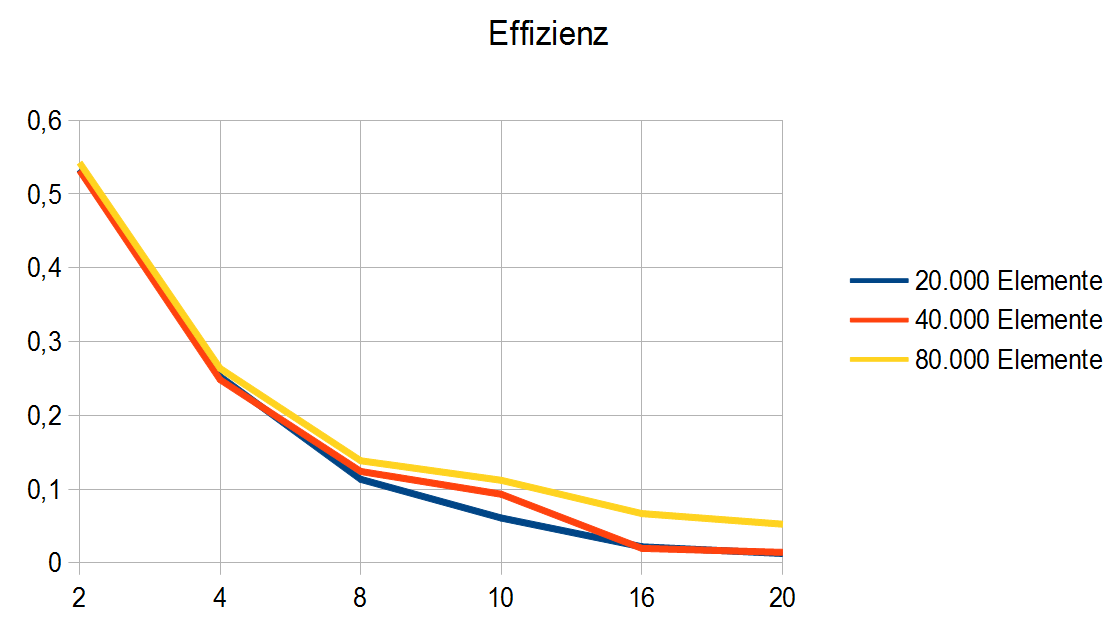
\includegraphics[width=1\hsize]{../effizienz.png}
  \end{center}
  \caption{\label{mpieffizienz}
    Effizienz-Diagramm f\"ur die MC-3-Implementierung mit der Funktion 1}
\end{figure}
\begin{figure}[htb]
  \begin{center}
    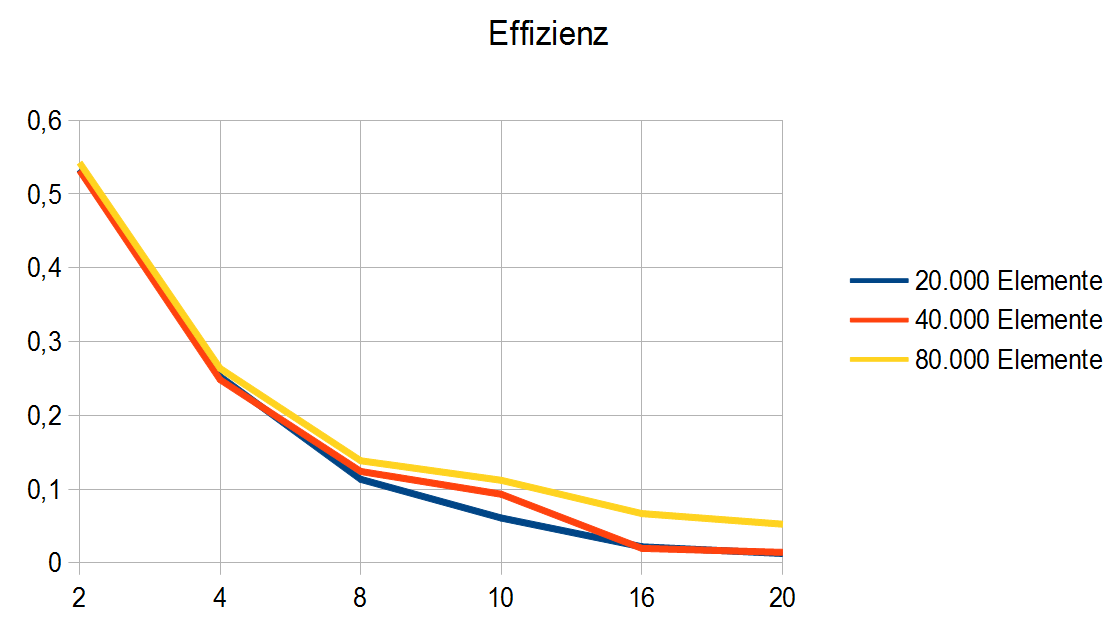
\includegraphics[width=1\hsize]{../effizienz.png}
  \end{center}
  \caption{\label{mpieffizienz}
    Effizienz-Diagramm f\"ur die MC-3-Implementierung mit der Funktion 2}
\end{figure}
Eine weiterer aussagekräftiger Wert ist die Effizienz.
Die Effizienz gibt die relative Verbesserung in der Verarbeitungsleistung an und ergibt sich aus dem Quotient von Speedup und Prozessoranzahl.
Wie aus dem betreffenden Diagramm ersichtlich wird, nimmt die Effizienz umgekehrt proportional zur Anzahl der eingesetzten
Prozessoren ab. Dabei hat die Anzahl der zu sortierenden Elemente nur marginalen Einfluss auf die jeweiligen Effizienzwerte.

\subsubsection{Kommunikationsanteil}
\begin{figure}[htb]
  \begin{center}
    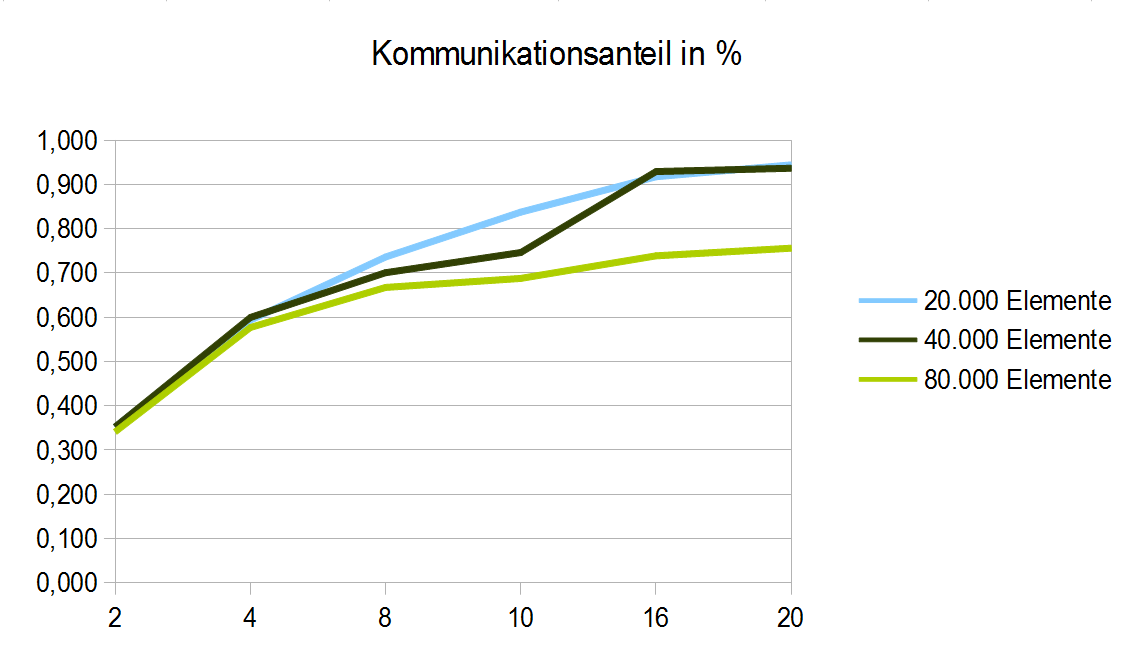
\includegraphics[width=1\hsize]{../Kommunikationsanteil.PNG}
  \end{center}
  \caption{\label{mpikommoverhead}
    Diagramm des Kommunikationsanteils f\"ur die MC3-Implementierung mit der Funktion 1}
\end{figure}
\begin{figure}[htb]
  \begin{center}
    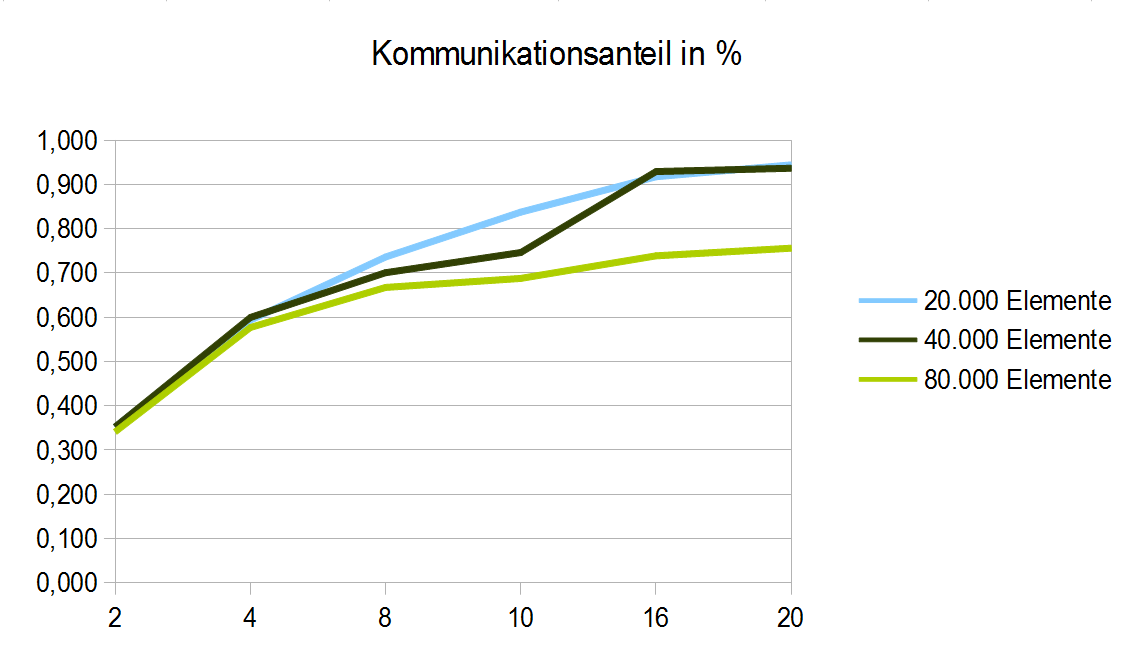
\includegraphics[width=1\hsize]{../Kommunikationsanteil.PNG}
  \end{center}
  \caption{\label{mpikommoverhead}
    Diagramm des Kommunikationsanteils f\"ur die MC3-Implementierung mit der Funktion 2}
\end{figure}
Die Auswertung der Messwerte zeigt, dass mit steigender Anzahl zu sortierender Elemente der Kommunikationsanteil an der Gesamtlaufzeit exponentiell ansteigt.
Bereits bei Verwendung von 8 Prozessoren betr\"agt der Kommunikationsanteil an der Gesamtlaufzeit etwa 70 Prozent und steigt weiter an, sodass schon
f\"ur 20 Prozessoren der Kommunikationsanteil \"uber 80 Prozent mit weiterhin steigender Tendenz betr\"agt.
Dieser hohe Anteil der Kommunikation an der Gesamtlaufzeit ist durch die in 2.4.2 aufgez\"ahlten Einflussfaktoren, besonders aber auf die Netzwerkstruktur und
und MPI Implementierung, zur\"uckzuf\"uhren.\\\\

Zusammenfassend kann die Aussage getroffen werden, dass die Implementierung des Merge-Splittung-Sort Algorithmus unter der MPI-Umgebung nicht geeignet ist.\\
Die unter bestimmten Voraussetzungen zu erreichende maginale Verk\"urzung der Gesamtlaufzeit ist gering, sodass vor der konkreten Nutzung dieser
Implementierung im vornherein betrachtet werden muss, ob die Anzahl der Prozessoren und zu sortierenden Elemente zu einer Verbesserung der Gesamtlaufzeit
f\"uhrt.

\subsubsection{Genauigkeit der Funktionen}
\begin{figure}[htb]
  \begin{center}
    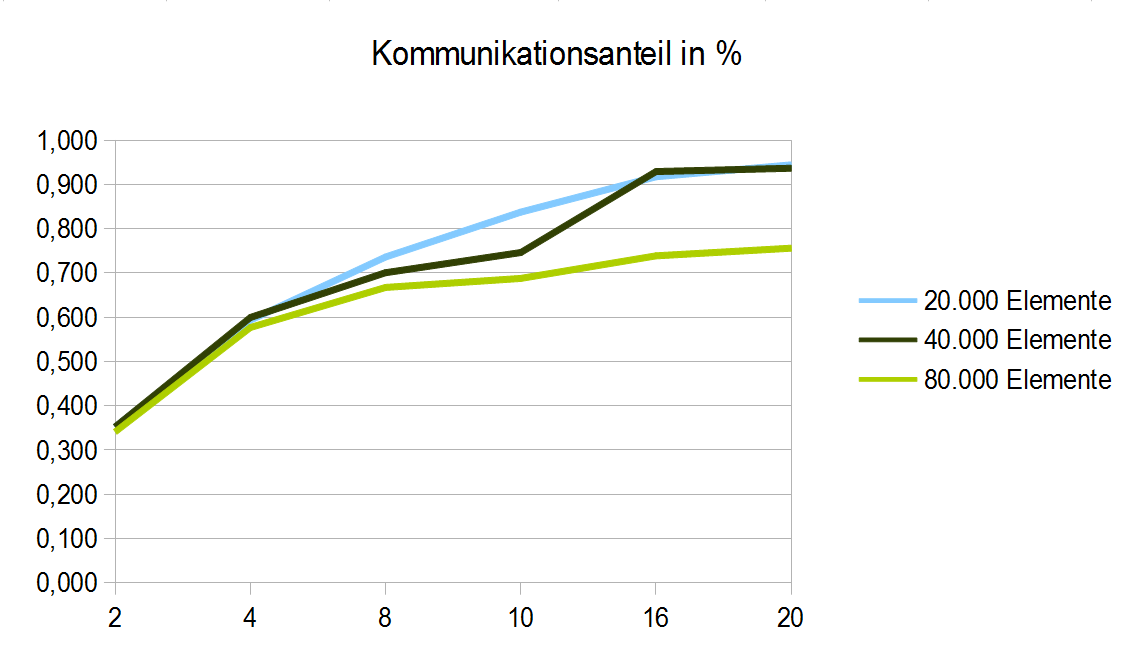
\includegraphics[width=1\hsize]{../Kommunikationsanteil.PNG}
  \end{center}
  \caption{\label{mpikommoverhead}
    Diagramm der Abweichung von $\pi$ der Funktion 1}
\end{figure}
\begin{figure}[htb]
  \begin{center}
    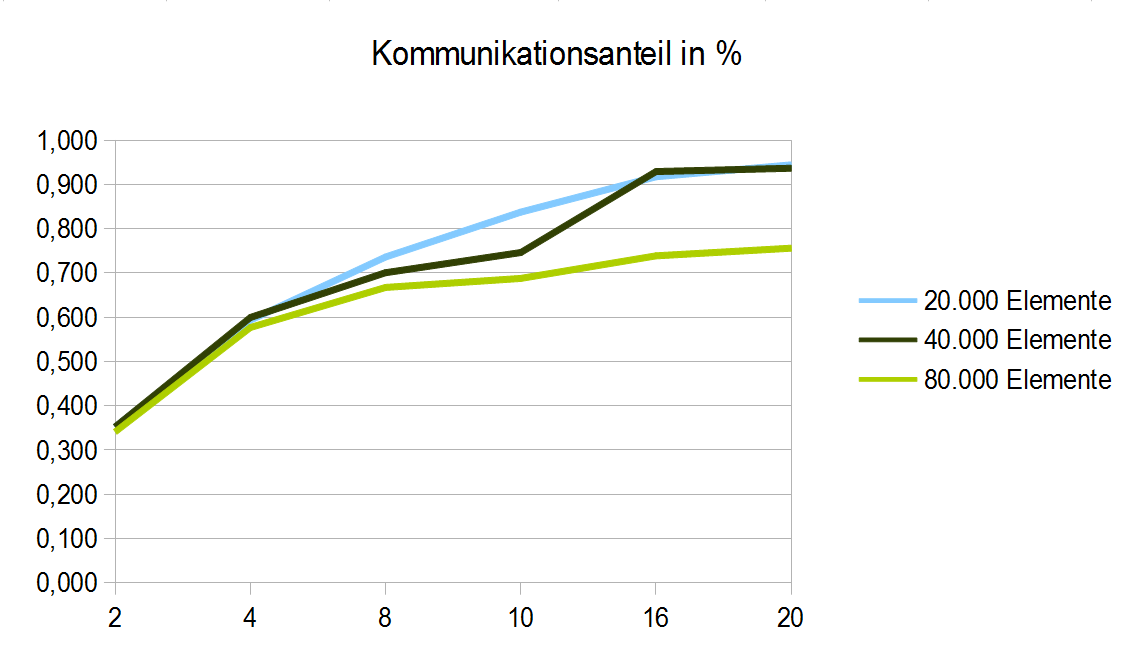
\includegraphics[width=1\hsize]{../Kommunikationsanteil.PNG}
  \end{center}
  \caption{\label{mpikommoverhead}
    Diagramm der Abweichung von $\pi$ der Funktion 2}
\end{figure}


\section{Anhang}
\subsection{Quellcode-Listings MPI}
\definecolor{listinggray}{gray}{0.9}
\definecolor{lbcolor}{rgb}{0.9,0.9,0.9}
\lstset{
	language=BASH,
	keywordstyle=\bfseries\ttfamily\color[rgb]{0,0,1},
	identifierstyle=\ttfamily,
	commentstyle=\color[rgb]{0.133,0.545,0.133},
	stringstyle=\ttfamily\color[rgb]{0.627,0.126,0.941},
	showstringspaces=false,
	basicstyle=\scriptsize,
	numbers=left,
	stepnumber=1,
	numbersep=6pt,
	numberstyle=\tiny,
	tabsize=1,
	breaklines=true,	%automatischer Zeilenumbruch
	prebreak = \raisebox{0ex}[0ex][0ex]{\ensuremath{\hookleftarrow}},
	breakatwhitespace=false,
	aboveskip={1.5\baselineskip},
  	columns=fixed,
  	upquote=true,
  	extendedchars=true,
  	backgroundcolor=\color[rgb]{0.97,0.97,0.97},
}
\begin{lstlisting}[captionpos=b, caption=MPI BASH-Script: run.sh, label=mpirunsh]
#!/bin/bash

##0##  process script args:
CPUCOUNT=0
VRANGE=0
INPUTFILENAME="cluster.c"
OUTPUTFILENAME="cluster"


function usage {
  echo "Usage: $0 -c CPUCOUNT -v VALUERANGE -i INPUTFILE -o OUTPUTFILE"
  exit 1;
}

##8 params required
if [ $# -ne 8 ] ; then	## erzwinge die Angabe aller Startparameter
  usage;
fi

##process args
while getopts c:hi:o:v: opt
do
  case "$opt" in
    c) CPUCOUNT=$OPTARG;;
    h) usage;;
    i) INPUTFILENAME=$OPTARG;;
    o) OUTPUTFILENAME=$OPTARG;;
    v) VRANGE=$OPTARG;;
    \?) usage;;
  esac
done
echo "CPUCOUNT: $CPUCOUNT"
echo "VRANGE:   $VRANGE"
echo "INPUT:    $INPUTFILENAME"
echo "OUT:      $OUTPUTFILENAME"


##1##  compile
echo "STAGE 1 - compiling $INPUTFILENAME ..."
mpicc -Wall -o $OUTPUTFILENAME $INPUTFILENAME


##2## create hostlist dynamically
echo "STAGE 2 - creating host list ..."
HOSTLISTFILENAME="load.txt"

##remove already existing file without warning
touch $HOSTLISTFILENAME         ## create file if not already there
rm $HOSTLISTFILENAME            ## remove file

##ssh trough simson clients for every pingable simson
for i in 01 02 03 04 05 06 07 08 09 {10..24}
do
  ping -c 1 simson$i  > /dev/null
  if [ $? = 0 ]
  then
	## check per ssh cat /proc/loadavg and check with regex
    echo "`ping -c 1 simson${i} | grep "64 bytes" | awk ' BEGIN {FS="("} {print $2}' | awk ' BEGIN {FS=")"} {print $1}'` `ssh simson${i} cat
/proc/loadavg`" | grep -v -E '141.57.9.[0-9]{2} $' >> $HOSTLISTFILENAME
  fi
done
HOSTNR=`wc -l $HOSTLISTFILENAME | awk '{print $1}'`		## zaehle Anzahl erreichbarer Hosts

##remove already existing file without warning
touch $HOSTLISTFILENAME.sorted         ## create file if not already there
rm $HOSTLISTFILENAME.sorted            ## remove file

echo "Sortiere ${HOSTNR} Hosts nach Auslastung ..."
sort -k 2 $HOSTLISTFILENAME >> $HOSTLISTFILENAME.sorted
awk '{print $1}' $HOSTLISTFILENAME.sorted > $HOSTLISTFILENAME

echo "Zur Ausfuehrung werde folgenden ${CPUCOUNT} Hosts benutzt, da diese derzeit die geringste Auslastung haben:"
head -n ${CPUCOUNT} ${HOSTLISTFILENAME}.sorted > head.list
awk '{print "Node: " $1 " - Load on this Node:   " $2 " (avg last min)   " $3 " (avg last 5 min)   " $4 " (avg last 15 min) "}' head.list

sleep 1

##3## run program on this hosts
echo "STAGE 3 - run $OUTPUTFILENAME on $CPUCOUNT cpus "
mpirun -np $CPUCOUNT -hostfile $HOSTLISTFILENAME $OUTPUTFILENAME $VRANGE

##cleanup - remove temporary used files
#rm $HOSTLISTFILENAME
#rm $HOSTLISTFILENAME.sorted
\end{lstlisting}

\definecolor{listinggray}{gray}{0.9}
\definecolor{lbcolor}{rgb}{0.9,0.9,0.9}
\lstset{
	language=BASH,
	keywordstyle=\bfseries\ttfamily\color[rgb]{0,0,1},
	identifierstyle=\ttfamily,
	commentstyle=\color[rgb]{0.133,0.545,0.133},
	stringstyle=\ttfamily\color[rgb]{0.627,0.126,0.941},
	showstringspaces=false,
	basicstyle=\scriptsize,
	numbers=left,
	stepnumber=1,
	numbersep=6pt,
	numberstyle=\tiny,
	tabsize=1,
	breaklines=true,	%automatischer Zeilenumbruch
	prebreak = \raisebox{0ex}[0ex][0ex]{\ensuremath{\hookleftarrow}},
	breakatwhitespace=false,
	aboveskip={1.5\baselineskip},
  	columns=fixed,
  	upquote=true,
  	extendedchars=true,
  	backgroundcolor=\color[rgb]{0.97,0.97,0.97},
}
\begin{lstlisting}[captionpos=b, caption=MPI BASH-Script: bench.sh, label=mpibenchsh]
#!/bin/bash

## Initial run.sh aufrufen um Auslastung der Pool-Rechner zum jetzigen Zeitpunkt zu ermitteln
./run.sh -c 20 -v 20 -i cluster.c -o cluster

for val in 20000 40000 80000	# Anzahl der zu messenden n Elemente
do
  for cpu in 2 4 8 10 16 20		# fuer p Prozessoren
  do							# jeweils 5 Messungen
	  mpirun -np $cpu -hostfile load.txt cluster $val
	  mpirun -np $cpu -hostfile load.txt cluster $val
	  mpirun -np $cpu -hostfile load.txt cluster $val
	  mpirun -np $cpu -hostfile load.txt cluster $val
	  mpirun -np $cpu -hostfile load.txt cluster $val
  done
done
\end{lstlisting}


\subsection{Quellcode-Listings MC-3}
\label{mc3:erfassungsh}
\definecolor{listinggray}{gray}{0.9}
\definecolor{lbcolor}{rgb}{0.9,0.9,0.9}
\lstset{
	language=BASH,
	keywordstyle=\bfseries\ttfamily\color[rgb]{0,0,1},
	identifierstyle=\ttfamily,
	commentstyle=\color[rgb]{0.133,0.545,0.133},
	stringstyle=\ttfamily\color[rgb]{0.627,0.126,0.941},
	showstringspaces=false,
	basicstyle=\scriptsize,
	numbers=left,
	stepnumber=1,
	numbersep=6pt,
	numberstyle=\tiny,
	tabsize=1,
	breaklines=true,	%automatischer Zeilenumbruch
	prebreak = \raisebox{0ex}[0ex][0ex]{\ensuremath{\hookleftarrow}},
	breakatwhitespace=false,
	aboveskip={1.5\baselineskip},
  	columns=fixed,
  	upquote=true,
  	extendedchars=true,
  	backgroundcolor=\color[rgb]{0.97,0.97,0.97},
}
\begin{lstlisting}[captionpos=b, caption=MC-3 BASH-Script: erfassung.sh, label=mc3erfassungsh]
#!/bin/bash
echo 'Prozessoranzahl;Intervalle;Laufzeit;Speedup;Abweichung' > $1
for x in 2 ; do
	for y in 1 2 4; do
			for z in 1 2 4 8 16 32 64 128 256 512 1024 2048; do
				echo -n $(( $x*$y ))\;$z\; >> $1
				run -f1 $y $x mc3.px $z $2 >> $1
				echo '' >> $1
			done
	done
done
\end{lstlisting}




%Beginn einer neuen Seite
\clearpage

\section{Glossar}
\begin{description}
 \item[DHCP-Server] DHCP steht als Abk\"urzung f\"ur "Dynamic Host
Configuration Protokoll" und beschreibt Techniken um Hosts in Netzwerken
dynamisch Netzwerkparameter wie IP-Adressen zuzuwei\ss{}en\footnote{\cite{dhcp}}
 \item[Router] Ein Rechnersystem mit mindestens zwei Netzwerkschnittstellen,
das Netzwerkschverkehr zwischen diesen Netzwerkschnittstellen nach einem
Regelwerk vermittelt und weiterleitet.
 \item[Routerdistribution] Eine spezielle Art von Betriebssystem, deren
Hauptaugenmerk bei der Konzeption und Entwicklung darauf liegt
Router-Funktionen sicher und stabil auszuf\"uhren
 \item[VLAN] Die Abk\"urzung VLAN steht f\"ur Virtual Local Area Network und
fasst Techniken zusammen um physikale Netzwerkstrukturen logisch zu
Segmentieren, beispielsweise zur Erh\"ohung der Sicherheit oder um
Broadcast-Dom\"anen zu verkleinern.
\end{description}
\clearpage

\section{Literaturverzeichnis}

Musterfrau, Renate: Muster. Frankfurt 2003.


\begin{thebibliography}{99}

\bibitem{IPCopManual} http://www.ipcop.org/1.4.0/en/install/html/ , abrufbar am
16.12.2012

\end{thebibliography}
\end{document}
%% EOF
